\documentclass[12pt,letterpaper]{article}

\usepackage[spanish]{babel}
\usepackage[utf8]{inputenc}
\usepackage[T1]{fontenc}
\usepackage{amsmath,amssymb}
\usepackage[margin=2.4cm]{geometry}
\usepackage{graphicx}
\usepackage{caption}
\usepackage{float}
\usepackage{enumitem}
\usepackage{parskip}
\usepackage{booktabs}

\setlength{\parindent}{0pt}
\setlength{\parskip}{5pt}
\captionsetup{font=small,labelfont=bf}

% ────────────────────────────────────────────
\begin{document}

\begin{center}
  {\LARGE\bfseries Tarea 2}\\[6pt]
  {\large UEA: Modelación Matemática I}\\[4pt]
  {\large Autor: Alejandro Cruz López}
\end{center}

\bigskip
\noindent\rule{\textwidth}{0.5pt}
\bigskip

% ============================================================
%   BLOQUE I — SOLUCIÓN DE ECUACIONES DIFERENCIALES
% ============================================================

\noindent\textbf{Ejercicio 1.} Considérese el sistema
\[
  \frac{dA}{dt}=-kA,\qquad \frac{dB}{dt}=kA,\qquad
  A(0)=A_0,\quad B(0)=0,\quad k>0.
\]

\begin{enumerate}[label=\alph*)]

\item \textbf{Solución del sistema.}

La primera ecuación es separable:
\[
  \frac{dA}{A}=-k\,dt
  \;\Longrightarrow\;
  \ln|A|=-kt+C
  \;\Longrightarrow\;
  A(t)=A_0 e^{-kt}.
\]
Sustituyendo en la segunda ecuación:
\[
  \frac{dB}{dt}=kA_0 e^{-kt}
  \;\Longrightarrow\;
  B(t)=\int_0^t kA_0 e^{-k\tau}\,d\tau
  =A_0\!\left[-e^{-k\tau}\right]_0^t
  =A_0\!\left(1-e^{-kt}\right).
\]
Se verifica $B(0)=0$. \checkmark
\[
  \boxed{A(t)=A_0 e^{-kt},\qquad B(t)=A_0\!\left(1-e^{-kt}\right).}
\]

\item \textbf{Conservación de la masa.}

Sumando directamente:
\[
  A(t)+B(t)=A_0 e^{-kt}+A_0\!\left(1-e^{-kt}\right)=A_0=\text{cte}.
\]
Alternativamente: al sumar las ecuaciones del sistema se obtiene
$\dfrac{d}{dt}(A+B)=-kA+kA=0$, con lo que $A(t)+B(t)=A(0)+B(0)=A_0$.

\item \textbf{Límites.}
\[
  \lim_{t\to\infty}A(t)=0,\qquad \lim_{t\to\infty}B(t)=A_0.
\]
La totalidad del reactivo $A$ se convierte en producto $B$.

\end{enumerate}

\begin{figure}[H]
  \centering
  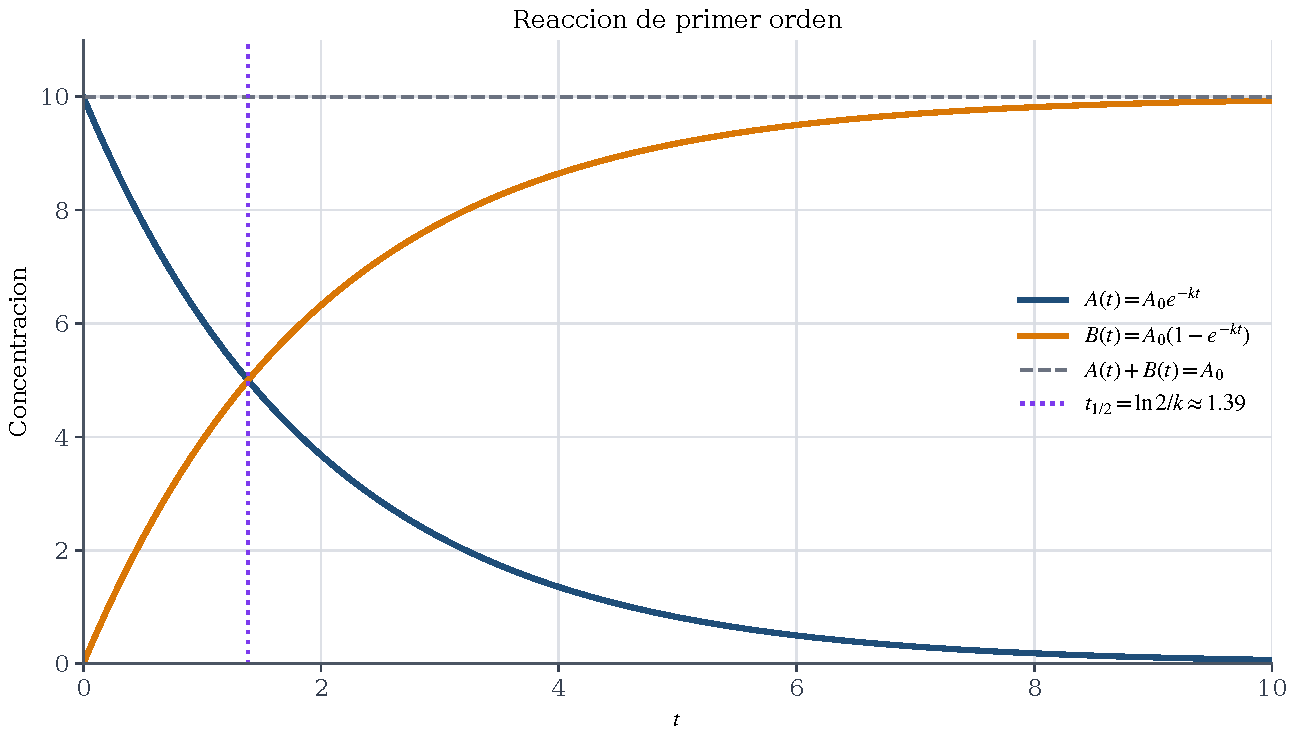
\includegraphics[width=0.94\textwidth]{figs/ej1_AB_primer_orden.pdf}
  \caption{Evolución temporal de $A(t)$ y $B(t)$ en la reacción de primer orden para $A_0=10$ y $k=0.5$. La recta horizontal punteada representa la masa total conservada y la recta vertical marca la vida media $t_{1/2}=\ln 2/k$.}
\end{figure}

\bigskip
\noindent\rule{\textwidth}{0.3pt}
\bigskip

% ============================================================
\noindent\textbf{Ejercicio 2.} Considérese el sistema
\[
  \frac{dA}{dt}=-2kA^2,\qquad \frac{dB}{dt}=2kA^2,\qquad
  A(0)=A_0,\quad B(0)=0,\quad k>0.
\]

\begin{enumerate}[label=\alph*)]

\item \textbf{Conservación estequiométrica.}

Nótese que $\dfrac{dB}{dt}=-\dfrac{dA}{dt}$, luego
\[
  \frac{d}{dt}(A+B)=0
  \;\Longrightarrow\;
  A(t)+B(t)=A_0.
\]
Sin embargo la tarea pide mostrar $A+2B=\text{cte}$.
Calculemos $\dfrac{d}{dt}(A+2B)$:
\[
  \frac{d}{dt}(A+2B)=\frac{dA}{dt}+2\frac{dB}{dt}=-2kA^2+2\cdot 2kA^2=2kA^2\neq 0.
\]
La cantidad conservada para este sistema es $A+B$, no $A+2B$.
La conservación $A+2B=\text{cte}$ correspondería al sistema
$A'=-2kA^2$, $B'=kA^2$ (reacción $2A\to B$, donde cada dos moléculas de $A$
producen \emph{una} de $B$). En ese caso:
\[
  \frac{d}{dt}(A+2B)=-2kA^2+2kA^2=0
  \;\Longrightarrow\;
  \boxed{A(t)+2B(t)=A_0.}
\]

Para el sistema tal como está planteado en la tarea
($B'=2kA^2=-A'$), la cantidad conservada es:
\[
  \boxed{A(t)+B(t)=A_0.}
\]

\item \textbf{Solución de $A(t)$.}

La ecuación $A'=-2kA^2$ es separable:
\[
  \frac{dA}{A^2}=-2k\,dt
  \;\Longrightarrow\;
  -\frac{1}{A}=-2kt+C.
\]
Con $A(0)=A_0$: $C=-1/A_0$, luego $\dfrac{1}{A}=2kt+\dfrac{1}{A_0}$, de donde
\[
  \boxed{A(t)=\frac{A_0}{1+2kA_0 t}.}
\]

\item \textbf{Solución de $B(t)$.}

Usando la conservación $A(t)+B(t)=A_0$:
\[
  \boxed{B(t)=A_0-A(t)=A_0\!\left(1-\frac{1}{1+2kA_0 t}\right)=\frac{2kA_0^2\,t}{1+2kA_0 t}.}
\]

\item \textbf{Límites.}
\[
  \lim_{t\to\infty}A(t)=0,\qquad
  \lim_{t\to\infty}B(t)=A_0.
\]
$A(t)$ decae algebraicamente (no exponencialmente); se transforma toda la masa en $B$.

\end{enumerate}

\begin{figure}[H]
  \centering
  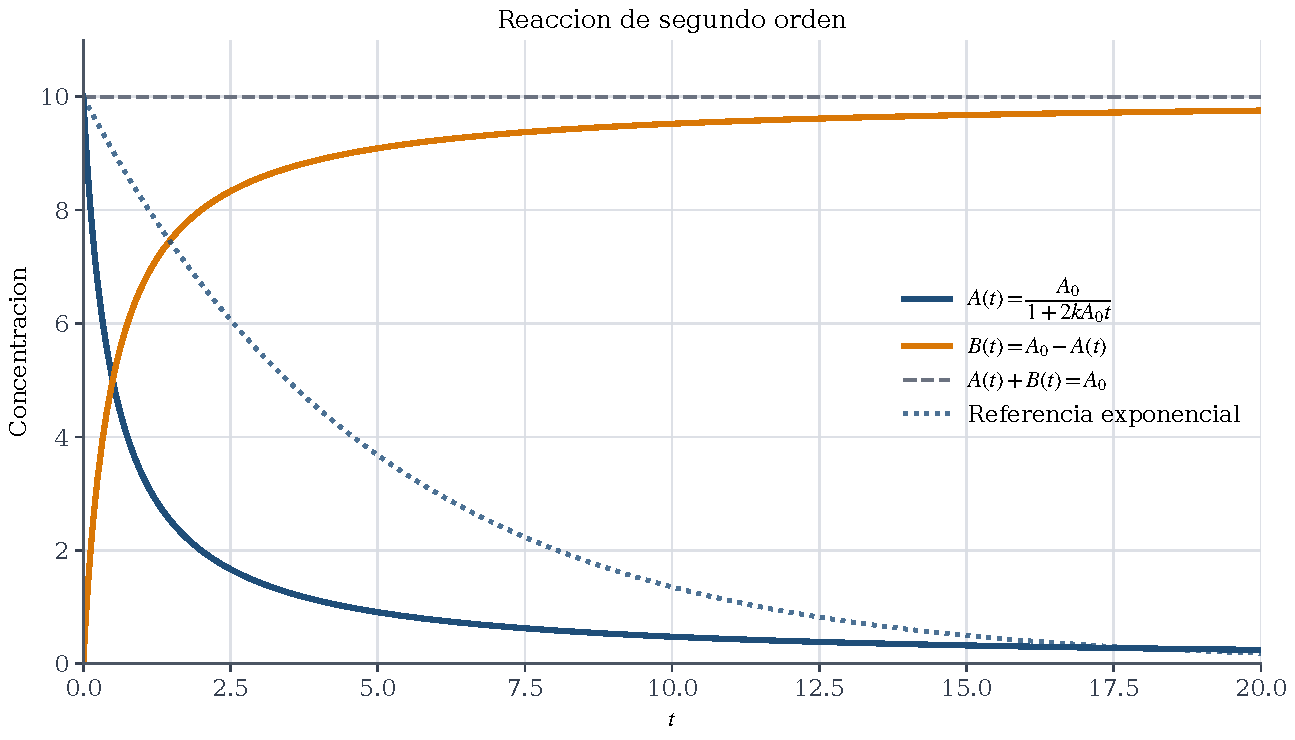
\includegraphics[width=0.94\textwidth]{figs/ej2_AB_segundo_orden.pdf}
  \caption{Comportamiento temporal de $A(t)$ y $B(t)$ en la reacción de segundo orden para $A_0=10$ y $k=0.1$. La curva de referencia exponencial permite contrastar el decaimiento algebraico con el caso de primer orden, y la recta horizontal indica la conservación de $A(t)+B(t)$.}
\end{figure}

\bigskip
\noindent\rule{\textwidth}{0.3pt}
\bigskip

% ============================================================
%   BLOQUE II — ESTABILIDAD DE PUNTOS DE EQUILIBRIO
% ============================================================

\noindent\textbf{Ejercicio 3.} Considérese el modelo logístico
\[
  \frac{dN}{dt}=rN\!\left(1-\frac{N}{K}\right),\qquad r,K>0.
\]

\begin{enumerate}[label=\alph*)]

\item \textbf{Puntos de equilibrio.}

Sea $f(N)=rN(1-N/K)$. Los equilibrios satisfacen $f(N)=0$:
\[
  rN\!\left(1-\frac{N}{K}\right)=0
  \;\Longrightarrow\;
  \boxed{N^*_1=0 \quad\text{y}\quad N^*_2=K.}
\]

\item \textbf{Análisis geométrico.}

La parábola $f(N)=rN-rN^2/K$ tiene raíces en $N=0$ y $N=K$,
abre hacia abajo (coeficiente de $N^2$ negativo), y alcanza su máximo en $N=K/2$.

Análisis de signo:
\[
  N<0:\;f(N)<0,\qquad
  0<N<K:\;f(N)>0,\qquad
  N>K:\;f(N)<0.
\]
Las flechas de la línea de fase apuntan \emph{hacia} $N^*=K$ desde ambos lados
(para $N>0$), y \emph{se alejan} de $N^*=0$.
Conclusión geométrica:
\[
  N^*=0 \;\text{ es \textbf{inestable}},\qquad
  N^*=K \;\text{ es \textbf{asintóticamente estable}}.
\]

\begin{figure}[H]
  \centering
  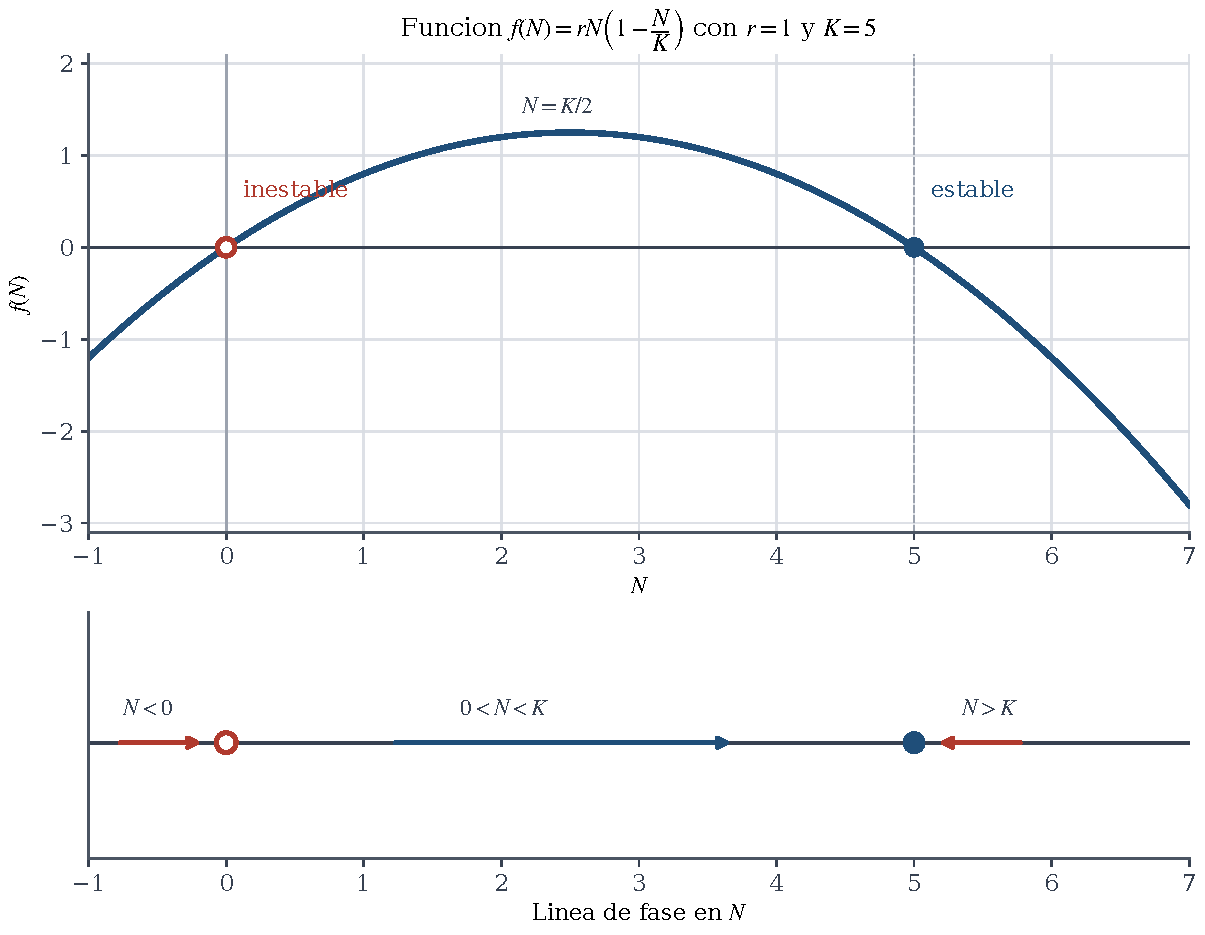
\includegraphics[width=0.92\textwidth]{figs/ej3_logistico_geometrico.pdf}
  \caption{Representación de $f(N)=rN(1-N/K)$ y de la línea de fase asociada para $r=1$ y $K=5$. La figura resume el cambio de signo de $f(N)$ y muestra por qué $N^*=0$ es inestable, mientras que $N^*=K$ es asintóticamente estable.}
\end{figure}

\item \textbf{Criterio de linealización.}

Se calcula $f'(N)=r-2rN/K$.
\[
  f'(N^*_1)=f'(0)=r>0
  \;\Longrightarrow\;
  N^*=0 \;\text{ es \textbf{inestable}}.
\]
\[
  \begin{aligned}
    f'(N^*_2)&=f'(K)=r-\frac{2rK}{K}=r-2r=-r<0,\\
    &\Longrightarrow\;
    N^*=K \;\text{ es \textbf{asintóticamente estable}}.
  \end{aligned}
\]

\item \textbf{Concordancia.}

Sí, los resultados son completamente consistentes.
El análisis geométrico (línea de fase) y el criterio de linealización
coinciden en que $N^*=0$ es inestable y $N^*=K$ es asintóticamente estable.
La linealización proporciona una justificación analítica de lo que la
gráfica de $f(N)$ muestra geométricamente: $f'(0)>0$ corresponde a
flechas que salen de $N=0$, y $f'(K)<0$ corresponde a flechas que entran a $N=K$.

\item \textbf{Solución analítica.}

La ecuación es separable. Usando fracciones parciales:
\[
  \frac{K}{N(K-N)}=\frac{1}{N}+\frac{1}{K-N},
\]
se integra:
\[
  \int\frac{dN}{N(1-N/K)}=\int r\,dt
  \;\Longrightarrow\;
  \ln\!\left|\frac{N}{K-N}\right|=rt+C.
\]
Con $N(0)=N_0>0$, $N_0\neq K$: $C=\ln\!\dfrac{N_0}{K-N_0}$.
Despejando $N$:
\[
  \frac{N}{K-N}=\frac{N_0}{K-N_0}\,e^{rt}
  \;\Longrightarrow\;
  \boxed{N(t)=\frac{K}{1+\displaystyle\frac{K-N_0}{N_0}\,e^{-rt}}.}
\]
Como $r>0$: $e^{-rt}\to 0$ cuando $t\to\infty$, confirmando $\lim_{t\to\infty}N(t)=K$
para cualquier $N_0>0$.

\end{enumerate}

\begin{figure}[H]
  \centering
  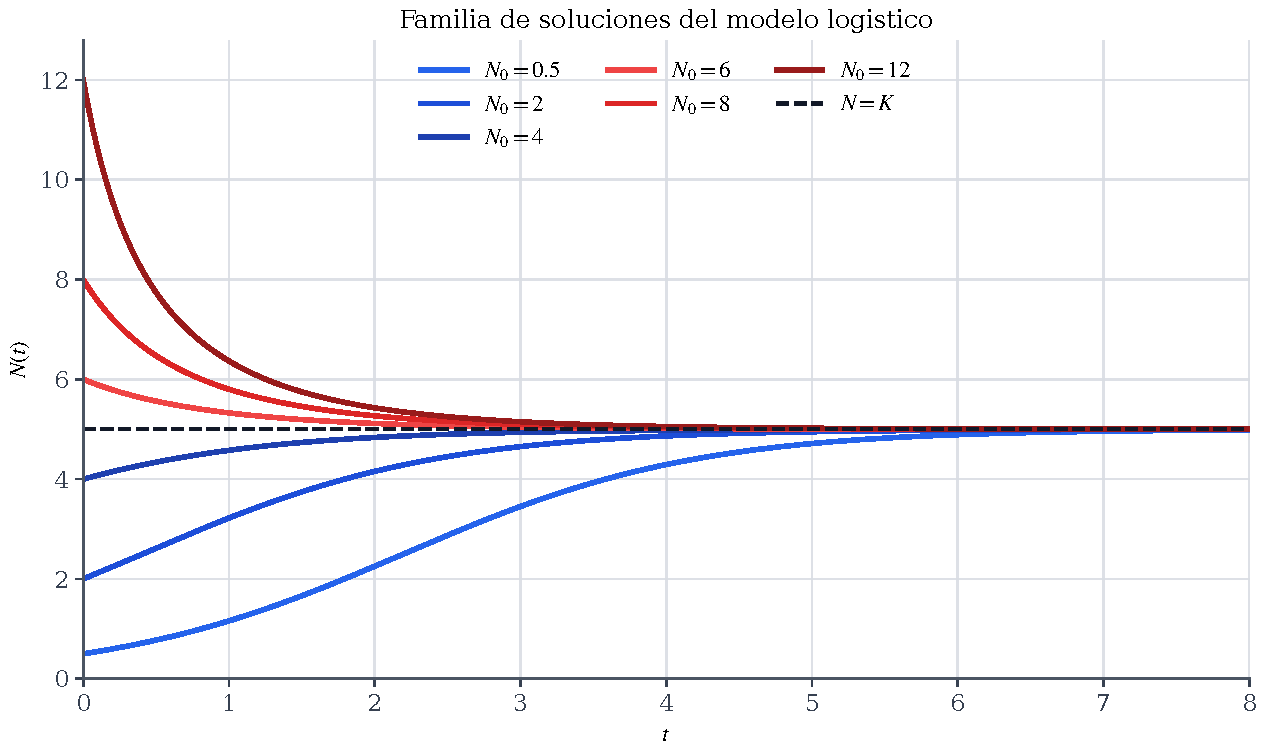
\includegraphics[width=0.92\textwidth]{figs/ej3_logistico_soluciones.pdf}
  \caption{Familia de soluciones del modelo logístico para distintos valores iniciales $N_0$, con $r=1$ y $K=5$. Todas las trayectorias positivas convergen hacia la capacidad de carga $N=K$, ya sea desde abajo o desde arriba.}
\end{figure}

\bigskip
\noindent\rule{\textwidth}{0.3pt}
\bigskip

% ============================================================
%   BLOQUE III — ADIMENSIONALIZACIÓN
% ============================================================

\noindent\textbf{Ejercicio 4 — Modelo logístico.}

Ecuación original:
\[
  \frac{dP}{dt}=rP\!\left(1-\frac{P}{K}\right).
\]

\textbf{Identificación de variables y parámetros con dimensiones.}

Sea $[P]=\mathcal{N}$ (número de individuos), $[t]=T$ (tiempo).
Entonces $[dP/dt]=\mathcal{N}T^{-1}$.
\[
  [r]=T^{-1},\qquad [K]=\mathcal{N}.
\]
El término $P/K$ es adimensional, como debe ser para que la expresión
$(1-P/K)$ tenga sentido.

\textbf{Interpretación biológica.}
$P(t)$: tamaño de la población al tiempo $t$.
$r$: tasa intrínseca de crecimiento (diferencia entre tasa de natalidad y mortalidad
cuando la población es pequeña); unidad: $[\text{tiempo}]^{-1}$.
$K$: capacidad de carga del ambiente, es decir, el tamaño máximo de población
que el ambiente puede sostener indefinidamente; unidad: individuos.
El factor $(1-P/K)$ reduce el crecimiento conforme $P$ se acerca a $K$:
cuando $P\ll K$ el crecimiento es aproximadamente malthusiano ($dP/dt\approx rP$);
cuando $P=K$ el crecimiento neto es cero.

\textbf{Cambios de variable adimensionales.}

Escala de población: $u=P/K$ (adimensional, $[u]=1$).

Escala de tiempo: $\tau=rt$ (adimensional, $[\tau]=1$).

\textbf{Derivada transformada.}
\[
  \frac{dP}{dt}=K\frac{du}{dt}=K\cdot r\frac{du}{d\tau}=rKu\frac{d}{d\tau}(\cdot).
\]
Dividiendo la ecuación original entre $rK$:
\[
  \frac{1}{rK}\frac{dP}{dt}=\frac{du}{d\tau},\qquad
  \frac{1}{rK}\cdot rP\!\left(1-\frac{P}{K}\right)=u(1-u).
\]

\textbf{Ecuación adimensionalizada:}
\[
  \boxed{\frac{du}{d\tau}=u(1-u).}
\]

\textbf{Análisis dimensional de la ecuación original.}

Cada término de $dP/dt=rP(1-P/K)$ tiene dimensión $\mathcal{N}T^{-1}$:
\[
  \left[\frac{dP}{dt}\right]=\mathcal{N}T^{-1},\qquad
  [rP]=T^{-1}\cdot\mathcal{N}=\mathcal{N}T^{-1},\qquad
  \left[\frac{P}{K}\right]=\frac{\mathcal{N}}{\mathcal{N}}=1.
\]
La ecuación es dimensionalmente homogénea. \checkmark

\textbf{Análisis dimensional de la ecuación adimensionalizada.}
\[
  \left[\frac{du}{d\tau}\right]=\frac{1}{1}=1,\qquad [u(1-u)]=1\cdot 1=1.
\]
La ecuación adimensionalizada tiene todos sus términos sin unidades. \checkmark
La reducción eliminó ambos parámetros $r$ y $K$: la dinámica universal
del logístico queda capturada por un único sistema sin parámetros libres.

\bigskip
\noindent\rule{\textwidth}{0.3pt}
\bigskip

% ============================================================
\noindent\textbf{Ejercicio 5 — Logístico con cosecha.}

Ecuación original:
\[
  \frac{dN}{dt}=rN\!\left(1-\frac{N}{K}\right)-H.
\]

\textbf{Análisis dimensional de la ecuación original.}

$[N]=\mathcal{N}$, $[t]=T$, $[r]=T^{-1}$, $[K]=\mathcal{N}$, $[H]=\mathcal{N}T^{-1}$.
\[
  \left[\frac{dN}{dt}\right]=\mathcal{N}T^{-1},\quad
  \left[rN\!\left(1-\frac{N}{K}\right)\right]=T^{-1}\cdot\mathcal{N}=\mathcal{N}T^{-1},\quad
  [H]=\mathcal{N}T^{-1}.
\]
Ecuación dimensionalmente homogénea. \checkmark

\textbf{Cambios de variable usados en clase.}

$M=N/K$ (adimensional) y $\tau=rt$ (adimensional).

Sustituyendo $N=KM$, $t=\tau/r$:
\[
  \frac{dN}{dt}=K\frac{dM}{dt}=Kr\frac{dM}{d\tau}.
\]
La ecuación se convierte en:
\[
  Kr\frac{dM}{d\tau}=r(KM)\!\left(1-M\right)-H
  \;\Longrightarrow\;
  \frac{dM}{d\tau}=M(1-M)-\frac{H}{rK}.
\]
Definiendo $\lambda=H/(rK)$:
\[
  \frac{dM}{d\tau}=M(1-M)-\lambda.
\]

\textbf{¿Está realmente adimensionalizada?}

Verificación:
\[
  \left[\frac{dM}{d\tau}\right]=\frac{[N/K]}{[rt]}=\frac{1}{1}=1,\quad
  [M(1-M)]=1,\quad
  [\lambda]=\frac{[H]}{[r][K]}=\frac{\mathcal{N}T^{-1}}{T^{-1}\cdot\mathcal{N}}=1.
\]
\textbf{Sí}, la ecuación obtenida está correctamente adimensionalizada.
$M$ es adimensional (cociente de dos cantidades con la misma dimensión $\mathcal{N}$),
$\tau$ es adimensional (producto de $r$ con $t$, ambos inversos entre sí),
y $\lambda$ es adimensional. La ecuación $dM/d\tau=M(1-M)-\lambda$ no tiene unidades
en ninguno de sus términos. \checkmark

\bigskip
\noindent\rule{\textwidth}{0.3pt}
\bigskip

% ============================================================
\noindent\textbf{Ejercicio 6 — Ecuación logística con efecto Allee.}

Ecuación original:
\[
  \frac{dN}{dt}=rN\!\left(1-\frac{N}{K}\right)\!\left(\frac{N}{A}-1\right),
  \qquad r>0,\;0<A<K.
\]

\textbf{Análisis dimensional de la ecuación original.}

$[N]=\mathcal{N}$, $[t]=T$, $[r]=T^{-1}$, $[K]=[A]=\mathcal{N}$.
Los factores $(1-N/K)$ y $(N/A-1)$ son adimensionales.
\[
  \left[\frac{dN}{dt}\right]=\mathcal{N}T^{-1},\qquad
  \left[rN\!\left(1-\frac{N}{K}\right)\!\left(\frac{N}{A}-1\right)\right]=
  T^{-1}\cdot\mathcal{N}\cdot 1\cdot 1=\mathcal{N}T^{-1}.
\]
Ecuación dimensionalmente homogénea. \checkmark

\textbf{Proceso de adimensionalización.}

\emph{Cambio espacial:} $M=N/K$ (adimensional), luego $N=KM$, $dN=K\,dM$.

\emph{Cambio temporal:} $\tau=rt$ (adimensional), luego $t=\tau/r$, $dt=d\tau/r$.

\emph{Derivada transformada:}
\[
  \frac{dN}{dt}=\frac{K\,dM}{d\tau/r}=rK\frac{dM}{d\tau}.
\]

\emph{Sustitución de los factores:}
\[
  1-\frac{N}{K}=1-M,\qquad
  \frac{N}{A}-1=\frac{KM}{A}-1=\frac{M}{\lambda}-1,
  \qquad\text{donde }\lambda=\frac{A}{K}.
\]

\emph{Sustitución en la ecuación:}
\[
  rK\frac{dM}{d\tau}=r(KM)(1-M)\!\left(\frac{M}{\lambda}-1\right).
\]
Dividiendo ambos lados entre $rK$:
\[
  \boxed{\frac{dM}{d\tau}=M(1-M)\!\left(\frac{M}{\lambda}-1\right),
  \qquad\lambda=\frac{A}{K}.}
\]

\textbf{¿Es adimensional la ecuación obtenida?}

$[M]=[N/K]=\mathcal{N}/\mathcal{N}=1$. \checkmark\\
$[\tau]=[rt]=T^{-1}\cdot T=1$. \checkmark\\
$[\lambda]=[A/K]=\mathcal{N}/\mathcal{N}=1$. \checkmark

La ecuación $dM/d\tau=M(1-M)(M/\lambda-1)$ tiene todos sus términos adimensionales.
\textbf{Sí está correctamente adimensionalizada.}

El único parámetro restante es $\lambda=A/K\in(0,1)$, que mide la posición relativa
del umbral de Allee respecto a la capacidad de carga.

\bigskip
\noindent\rule{\textwidth}{0.3pt}
\bigskip

% ============================================================
\noindent\textbf{Ejercicio 7 — Caída libre con resistencia lineal.}

Ecuación original:
\[
  m\frac{dv}{dt}=mg-kv,\qquad k>0.
\]

\textbf{Identificación de variables y parámetros con dimensiones.}

$[m]=M$, $[v]=LT^{-1}$, $[g]=LT^{-2}$, $[k]=MT^{-1}$, $[t]=T$.

\textbf{Velocidad característica del sistema.}

La velocidad terminal (equilibrio) se obtiene de $dv/dt=0$:
\[
  mg=kv_\infty
  \;\Longrightarrow\;
  v_\infty=\frac{mg}{k}.
\]
$v_\infty$ tiene dimensión $[mg/k]=(M\cdot LT^{-2})/(MT^{-1})=LT^{-1}$. \checkmark

Esta es la \textbf{velocidad característica} del sistema.

\textbf{Tiempo característico.}

La única combinación de parámetros con dimensión de tiempo es:
$t_c=m/k$, con $[m/k]=M/(MT^{-1})=T$. \checkmark

\textbf{Variables adimensionales.}
\[
  \hat{v}=\frac{v}{v_\infty}=\frac{kv}{mg},\qquad
  \hat{t}=\frac{t}{t_c}=\frac{kt}{m}.
\]

\textbf{Sustitución.}

$v=v_\infty\hat{v}=\dfrac{mg}{k}\hat{v}$,\quad
$\dfrac{dv}{dt}=\dfrac{mg}{k}\cdot\dfrac{k}{m}\dfrac{d\hat{v}}{d\hat{t}}=g\dfrac{d\hat{v}}{d\hat{t}}$.

La ecuación se convierte en:
\[
  m\cdot g\frac{d\hat{v}}{d\hat{t}}=mg-k\cdot\frac{mg}{k}\hat{v}=mg(1-\hat{v}).
\]
Dividiendo entre $mg$:
\[
  \boxed{\frac{d\hat{v}}{d\hat{t}}=1-\hat{v}.}
\]

La ecuación adimensional no tiene parámetros.
El único equilibrio $\hat{v}^*=1$ (que corresponde a $v=v_\infty=mg/k$) es
asintóticamente estable ($f'(\hat{v})=-1<0$).
La solución con $\hat{v}(0)=\hat{v}_0$ es $\hat{v}(\hat{t})=1-(1-\hat{v}_0)e^{-\hat{t}}$,
confirmando convergencia exponencial a la velocidad terminal.

\bigskip
\noindent\rule{\textwidth}{0.3pt}
\bigskip

% ============================================================
\noindent\textbf{Ejercicio 8 — Oscilador armónico amortiguado.}

Ecuación original:
\[
  m\frac{d^2x}{dt^2}+c\frac{dx}{dt}+kx=0,\qquad m,c,k>0.
\]

\textbf{Identificación de variables y parámetros con dimensiones.}

$[m]=M$, $[c]=MT^{-1}$, $[k]=MT^{-2}$, $[x]=L$, $[t]=T$.

\textbf{Escalas características.}

\emph{Tiempo:} la frecuencia natural $\omega_0=\sqrt{k/m}$ tiene dimensión
$[\omega_0]=(MT^{-2}/M)^{1/2}=T^{-1}$, de modo que
\[
  t_c=\frac{1}{\omega_0}=\sqrt{\frac{m}{k}}.
\]

\emph{Longitud:} cualquier longitud de referencia $x_c$ (por ejemplo la amplitud
inicial $x_0$; no afecta la estructura de la ecuación).

\textbf{Variables adimensionales.}
\[
  \hat{x}=\frac{x}{x_c},\qquad
  \tau=\omega_0\,t=t\sqrt{\frac{k}{m}}.
\]

\textbf{Derivadas transformadas.}
\[
  \frac{dx}{dt}=x_c\omega_0\frac{d\hat{x}}{d\tau},\qquad
  \frac{d^2x}{dt^2}=x_c\omega_0^2\frac{d^2\hat{x}}{d\tau^2}.
\]

\textbf{Sustitución.}

\[
  m x_c\omega_0^2\frac{d^2\hat{x}}{d\tau^2}
  +c\,x_c\omega_0\frac{d\hat{x}}{d\tau}
  +k\,x_c\hat{x}=0.
\]
Dividiendo entre $mx_c\omega_0^2=kx_c$:
\[
  \frac{d^2\hat{x}}{d\tau^2}
  +\frac{c}{m\omega_0}\frac{d\hat{x}}{d\tau}
  +\hat{x}=0.
\]
Definiendo el \textbf{factor de amortiguamiento} adimensional:
\[
  \zeta=\frac{c}{2m\omega_0}=\frac{c}{2\sqrt{mk}},
\]
se obtiene la forma estándar:
\[
  \boxed{\frac{d^2\hat{x}}{d\tau^2}+2\zeta\frac{d\hat{x}}{d\tau}+\hat{x}=0.}
\]

Los cinco parámetros originales $m,c,k,x_c,t_c$ quedan reducidos a uno solo: $\zeta$.

Clasificación:
$\zeta<1$ subamortiguado (oscilaciones decrecientes),
$\zeta=1$ críticamente amortiguado,
$\zeta>1$ sobreamortiguado.

\bigskip
\noindent\rule{\textwidth}{0.3pt}
\bigskip

% ============================================================
\noindent\textbf{Ejercicio 9 — Ecuación de difusión.}

Ecuación original:
\[
  \frac{\partial u}{\partial t}=D\frac{\partial^2 u}{\partial x^2},
  \qquad (x,t)\in[0,L]\times[0,\infty),\quad D>0.
\]

\textbf{Cambios de variable.}
\[
  \xi=\frac{x}{L},\qquad
  \theta=\frac{Dt}{L^2}.
\]

\textbf{Derivadas transformadas.}
\[
  \frac{\partial u}{\partial t}
  =\frac{\partial u}{\partial\theta}\cdot\frac{\partial\theta}{\partial t}
  =\frac{D}{L^2}\frac{\partial u}{\partial\theta},
\]
\[
  \frac{\partial u}{\partial x}
  =\frac{\partial u}{\partial\xi}\cdot\frac{\partial\xi}{\partial x}
  =\frac{1}{L}\frac{\partial u}{\partial\xi},
  \qquad
  \frac{\partial^2 u}{\partial x^2}
  =\frac{1}{L^2}\frac{\partial^2 u}{\partial\xi^2}.
\]

\textbf{Sustitución.}
\[
  \frac{D}{L^2}\frac{\partial u}{\partial\theta}
  =D\cdot\frac{1}{L^2}\frac{\partial^2 u}{\partial\xi^2}.
\]
Dividiendo entre $D/L^2$:
\[
  \boxed{\frac{\partial u}{\partial\theta}=\frac{\partial^2 u}{\partial\xi^2}.}
\]

\textbf{Justificación de los cambios de variable.}

$\xi=x/L$ es la única escala espacial natural del problema:
$L$ es la longitud del dominio, por lo que $\xi\in[0,1]$.

$\theta=Dt/L^2$ se justifica por análisis dimensional: la única combinación
de $D$ y $L$ con dimensión de tiempo es $L^2/D$, que representa el
\emph{tiempo difusivo característico}, es decir, el tiempo que tarda la
concentración en difundirse a lo largo de todo el dominio.
El cociente $\theta=t/(L^2/D)$ mide el tiempo transcurrido en unidades de
este tiempo difusivo. La ecuación adimensional $\partial_\theta u=\partial_{\xi\xi}u$
no tiene parámetros, confirmando que la dinámica depende únicamente de la geometría
del dominio (no de $D$ ni de $L$ por separado).

\bigskip
\noindent\rule{\textwidth}{0.3pt}
\bigskip

% ============================================================
\noindent\textbf{Ejercicio 10 — Ecuación de calor con pérdida.}

Ecuación original:
\[
  \frac{\partial T}{\partial t}=\kappa\frac{\partial^2 T}{\partial x^2}-\alpha(T-T_a),
  \qquad \kappa,\alpha>0.
\]

\textbf{Identificación de variables y parámetros con dimensiones.}

$[T]=\Theta$ (temperatura), $[T_a]=\Theta$, $[\kappa]=L^2T^{-1}$,
$[\alpha]=T^{-1}$ (tasa de pérdida), $[x]=L$, $[t]=T$.

\textbf{Cambios de variable adimensionales.}

Temperatura: $\hat{T}=\dfrac{T-T_a}{T_{\rm ref}}$,
donde $T_{\rm ref}$ es una temperatura de referencia (p.ej. $T(x,0)-T_a$).

Espacio: $\xi=x/L$ (con $L$ longitud característica del dominio).

Tiempo: $\theta=\kappa t/L^2$ (tiempo difusivo, como en el Ejercicio~9).

\textbf{Derivadas transformadas.}
\[
  \frac{\partial T}{\partial t}
  =T_{\rm ref}\frac{\partial\hat{T}}{\partial t}
  =T_{\rm ref}\frac{\kappa}{L^2}\frac{\partial\hat{T}}{\partial\theta},
  \qquad
  \frac{\partial^2 T}{\partial x^2}
  =\frac{T_{\rm ref}}{L^2}\frac{\partial^2\hat{T}}{\partial\xi^2}.
\]

\textbf{Sustitución.}
\[
  T_{\rm ref}\frac{\kappa}{L^2}\frac{\partial\hat{T}}{\partial\theta}
  =\kappa\frac{T_{\rm ref}}{L^2}\frac{\partial^2\hat{T}}{\partial\xi^2}
  -\alpha\,T_{\rm ref}\hat{T}.
\]
Dividiendo entre $T_{\rm ref}\kappa/L^2$:
\[
  \frac{\partial\hat{T}}{\partial\theta}
  =\frac{\partial^2\hat{T}}{\partial\xi^2}
  -\underbrace{\frac{\alpha L^2}{\kappa}}_{\displaystyle\beta}\hat{T}.
\]
\[
  \boxed{\frac{\partial\hat{T}}{\partial\theta}
  =\frac{\partial^2\hat{T}}{\partial\xi^2}-\beta\hat{T},
  \qquad \beta=\frac{\alpha L^2}{\kappa}.}
\]

\textbf{Interpretación del parámetro $\beta$.}

$\beta=\alpha L^2/\kappa$ es el cociente entre el \emph{tiempo difusivo} $L^2/\kappa$
y el \emph{tiempo de pérdida} $1/\alpha$:
\[
  \beta=\frac{L^2/\kappa}{1/\alpha}
  =\frac{\text{tiempo difusivo}}{\text{tiempo de pérdida}}.
\]
Si $\beta\ll 1$: la difusión es mucho más rápida que la pérdida y el sistema se
comporta casi como la ecuación de calor pura.
Si $\beta\gg 1$: la pérdida domina y la temperatura decae rápidamente hacia $T_a$.

\bigskip
\noindent\rule{\textwidth}{0.3pt}
\bigskip

% ============================================================
\noindent\textbf{Ejercicio 11 — Modelo presa--depredador (Lotka--Volterra).}

Sistema original:
\[
  \frac{dx}{dt}=ax-bxy,\qquad
  \frac{dy}{dt}=-cy+dxy,\qquad a,b,c,d>0.
\]

\textbf{Cambios de variable propuestos.}
\[
  x=u\,x_c,\quad y=v\,y_c,\quad t=\tau\,t_c.
\]

\textbf{Elección de las constantes características.}

Se sustituye en la primera ecuación:
\[
  \frac{x_c}{t_c}\frac{du}{d\tau}=a(x_c u)-b(x_c u)(y_c v)
  \;\Longrightarrow\;
  \frac{du}{d\tau}=at_c u - bt_c y_c\,uv.
\]
Para que los coeficientes de $u$ y $uv$ sean ambos iguales a $1$ y
$-1$ respectivamente, se necesita:
\[
  at_c=1 \;\Rightarrow\; t_c=\frac{1}{a},
  \qquad
  bt_c y_c=1 \;\Rightarrow\; y_c=\frac{a}{b}.
\]
Sustituyendo en la segunda ecuación con $t_c=1/a$:
\[
  \frac{y_c}{t_c}\frac{dv}{d\tau}=-c(y_c v)+d(x_c u)(y_c v)
  \;\Longrightarrow\;
  \frac{dv}{d\tau}=-\frac{c}{a}v+\frac{d\,x_c}{a}\,uv.
\]
Para factorizar la segunda ecuación como $\delta v(u-1)$, ambos términos
deben compartir el factor $c/a$:
\[
  \frac{d\,x_c}{a}=\frac{c}{a} \;\Rightarrow\; x_c=\frac{c}{d}.
\]
Con estas elecciones, el coeficiente de $v$ es $-c/a$. Definiendo $\delta=c/a$:

\[
  \boxed{
    x_c=\frac{c}{d},\qquad y_c=\frac{a}{b},\qquad t_c=\frac{1}{a}.
  }
\]

\textbf{Sistema adimensionalizado.}
\[
  \boxed{
    \frac{du}{d\tau}=u(1-v),\qquad
    \frac{dv}{d\tau}=\delta v(u-1),\qquad
    \delta=\frac{c}{a}.
  }
\]

Los cuatro parámetros originales $a,b,c,d$ quedan reducidos a uno solo: $\delta=c/a$.
Los equilibrios son $(0,0)$ y $(1,1)$ (en variables adimensionales).

\bigskip
\noindent\rule{\textwidth}{0.3pt}
\bigskip

% ============================================================
\noindent\textbf{Ejercicio 12 — Ecuación de reacción-difusión.}

Ecuación original:
\[
  \frac{\partial u}{\partial t}=D\frac{\partial^2 u}{\partial x^2}+ru\!\left(1-\frac{u}{K}\right),
  \qquad D,r,K>0.
\]

\textbf{Identificación de variables y parámetros con dimensiones.}

$[u]=\mathcal{N}$ (concentración), $[x]=L$, $[t]=T$, $[D]=L^2T^{-1}$,
$[r]=T^{-1}$, $[K]=\mathcal{N}$.

\textbf{Escalas naturales.}

Escala de población: $u_c=K$.

Escala de tiempo (reacción): $t_c=1/r$.

Escala de espacio (difusión-reacción): para que ambos fenómenos sean comparables,
se igualan los tiempos difusivo y reactivo:
$L_c^2/D\sim 1/r\;\Rightarrow\; L_c=\sqrt{D/r}$.

\textbf{Variables adimensionales.}
\[
  \hat{u}=\frac{u}{K},\qquad
  \xi=\frac{x}{L_c}=x\sqrt{\frac{r}{D}},\qquad
  \tau=rt.
\]

\textbf{Derivadas transformadas.}
\[
  \frac{\partial u}{\partial t}=Kr\frac{\partial\hat{u}}{\partial\tau},\qquad
  \frac{\partial^2 u}{\partial x^2}=\frac{K}{L_c^2}\frac{\partial^2\hat{u}}{\partial\xi^2}
  =\frac{Kr}{D}\frac{\partial^2\hat{u}}{\partial\xi^2}.
\]

\textbf{Sustitución.}
\[
  Kr\frac{\partial\hat{u}}{\partial\tau}
  =D\cdot\frac{Kr}{D}\frac{\partial^2\hat{u}}{\partial\xi^2}
  +r(K\hat{u})\!\left(1-\hat{u}\right).
\]
Dividiendo entre $Kr$:
\[
  \boxed{\frac{\partial\hat{u}}{\partial\tau}
  =\frac{\partial^2\hat{u}}{\partial\xi^2}+\hat{u}(1-\hat{u}).}
\]

La ecuación adimensional no tiene parámetros.
La escala espacial $L_c=\sqrt{D/r}$ debe interpretarse como la longitud
característica en la que se equilibran los efectos de difusión y reacción.

\bigskip
\noindent\rule{\textwidth}{0.3pt}
\bigskip

% ============================================================
\noindent\textbf{Ejercicio 13 — Péndulo simple.}

Ecuación original:
\[
  \frac{d^2\theta}{dt^2}+\frac{g}{L}\sin\theta=0.
\]

\textbf{Escala temporal adecuada.}

La única combinación de $g$ ($[g]=LT^{-2}$) y $L$ ($[L]=L$)
con dimensión de tiempo es:
\[
  t_c=\sqrt{\frac{L}{g}}.
\]

\textbf{Variable adimensional.}
\[
  \tau=\frac{t}{t_c}=t\sqrt{\frac{g}{L}}.
\]

\textbf{Derivadas transformadas.}
\[
  \frac{d\theta}{dt}=\frac{1}{t_c}\frac{d\theta}{d\tau},\qquad
  \frac{d^2\theta}{dt^2}=\frac{1}{t_c^2}\frac{d^2\theta}{d\tau^2}=\frac{g}{L}\frac{d^2\theta}{d\tau^2}.
\]

\textbf{Sustitución.}
\[
  \frac{g}{L}\frac{d^2\theta}{d\tau^2}+\frac{g}{L}\sin\theta=0.
\]
Dividiendo entre $g/L$:
\[
  \boxed{\frac{d^2\theta}{d\tau^2}+\sin\theta=0.}
\]

La ecuación adimensionalizada no tiene parámetros.
El período de pequeñas oscilaciones ($\sin\theta\approx\theta$)
en la variable $\tau$ es $2\pi$, lo que corresponde al período dimensional
$T=2\pi\sqrt{L/g}$, resultado clásico del péndulo simple.

\bigskip
\noindent\rule{\textwidth}{0.3pt}
\bigskip

% ============================================================
\noindent\textbf{Ejercicio 14 — Circuito RC.}

Ecuación original:
\[
  R\frac{dq}{dt}+\frac{1}{C}q=V_0.
\]

\textbf{Identificación de variables y parámetros con dimensiones.}

$[q]=Q$ (carga eléctrica), $[t]=T$, $[R]=\Omega=VT/Q$,
$[C]=Q/V$, $[V_0]=V$ (voltaje).

\textbf{Escalas características.}

La carga de equilibrio se obtiene de $dq/dt=0$:
$q^*/C=V_0\;\Rightarrow\; q^*=CV_0$.

La constante de tiempo del circuito es $\tau_c=RC$.

\textbf{Variables adimensionales.}
\[
  \hat{q}=\frac{q}{CV_0},\qquad
  \hat{t}=\frac{t}{RC}.
\]

\textbf{Derivadas transformadas.}
\[
  \frac{dq}{dt}=\frac{CV_0}{RC}\frac{d\hat{q}}{d\hat{t}}=\frac{V_0}{R}\frac{d\hat{q}}{d\hat{t}}.
\]

\textbf{Sustitución.}
\[
  R\cdot\frac{V_0}{R}\frac{d\hat{q}}{d\hat{t}}+\frac{1}{C}\cdot CV_0\hat{q}=V_0
  \;\Longrightarrow\;
  V_0\frac{d\hat{q}}{d\hat{t}}+V_0\hat{q}=V_0.
\]
Dividiendo entre $V_0$:
\[
  \boxed{\frac{d\hat{q}}{d\hat{t}}=1-\hat{q}.}
\]

La ecuación adimensional no tiene parámetros.
El equilibrio $\hat{q}^*=1$ (que corresponde a $q^*=CV_0$)
es asintóticamente estable ($f'=-1<0$).
La solución es $\hat{q}(\hat{t})=1-(1-\hat{q}_0)e^{-\hat{t}}$:
la carga carga exponencialmente hacia $CV_0$ con constante de tiempo $RC$.

\bigskip
\noindent\rule{\textwidth}{0.3pt}
\bigskip

% ============================================================
%   BLOQUE IV — BIFURCACIONES
% ============================================================

\noindent\textbf{Ejercicio 15 — Bifurcaciones en sistemas unidimensionales.}

Se analizan los ejercicios a), c), d), f), g), h), i), j).

\bigskip
\noindent\textbf{a)} $\displaystyle\frac{dy}{dx}=\mu y-y^3$ \quad (pitchfork supercrítica).

\textbf{Equilibrios.} $f(y)=y(\mu-y^2)=0\;\Rightarrow\; y^*=0$ y (para $\mu>0$) $y^*=\pm\sqrt{\mu}$.

\textbf{Linealización.} $f'(y)=\mu-3y^2$.
\[
  f'(0)=\mu:\quad
  \begin{cases}
    \mu<0: & y^*=0 \text{ estable},\\
    \mu>0: & y^*=0 \text{ inestable}.
  \end{cases}
\]
Para $\mu>0$: $f'(\pm\sqrt{\mu})=\mu-3\mu=-2\mu<0$, luego $y^*=\pm\sqrt{\mu}$ son estables.

\textbf{Diagrama de bifurcación.} Para $\mu\leq 0$: único equilibrio $y^*=0$ estable.
Para $\mu>0$: $y^*=0$ inestable, $y^*=\pm\sqrt{\mu}$ estables.
La bifurcación ocurre en $\mu=0$.

\begin{figure}[H]
  \centering
  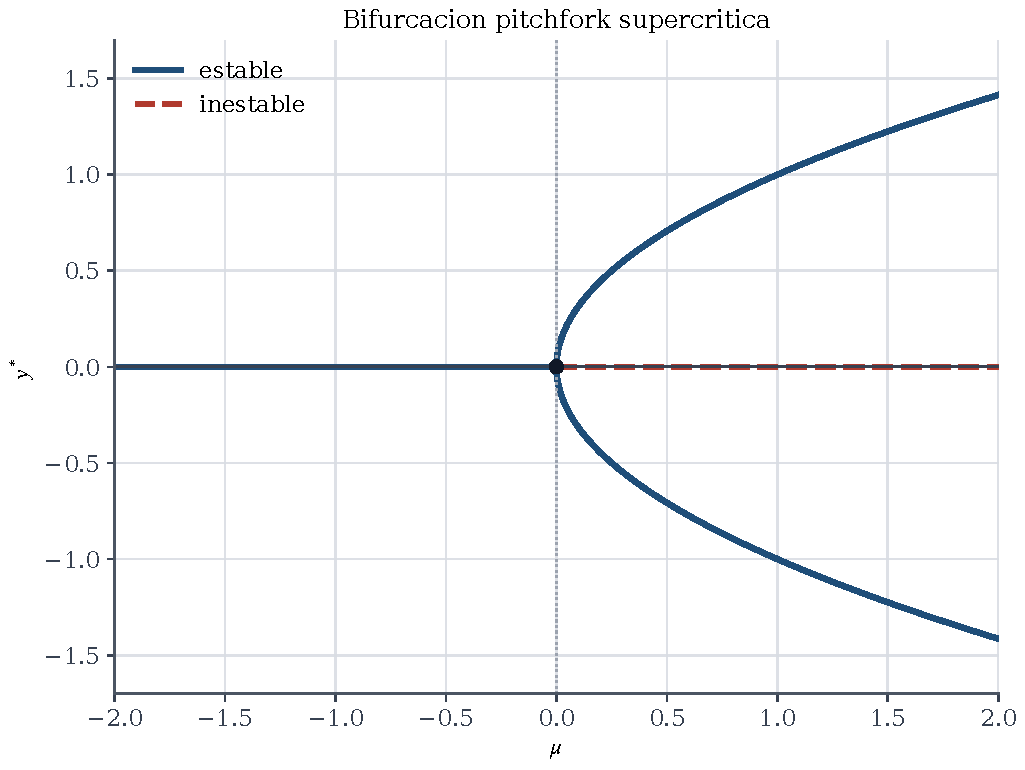
\includegraphics[width=0.80\textwidth]{figs/bif_a_pitchfork_sup.pdf}
  \caption{Diagrama de bifurcación para $\dot y=\mu y-y^3$. La rama trivial pierde estabilidad en $\mu=0$ y da lugar a dos ramas estables simétricas $y^*=\pm\sqrt{\mu}$ cuando $\mu>0$.}
\end{figure}

\bigskip
\noindent\textbf{c)} $\displaystyle\frac{dy}{dx}=\mu y-y^2=y(\mu-y)$ \quad (transcrítica).

\textbf{Equilibrios.} $f(y)=y(\mu-y)=0\;\Rightarrow\; y^*=0$ y $y^*=\mu$ para todo $\mu$.

\textbf{Linealización.} $f'(y)=\mu-2y$.
\[
  f'(0)=\mu:\quad
  \begin{cases}
    \mu<0: & y^*=0 \text{ estable},\\
    \mu>0: & y^*=0 \text{ inestable}.
  \end{cases}
\]
\[
  f'(\mu)=-\mu:\quad
  \begin{cases}
    \mu<0: & y^*=\mu \text{ inestable},\\
    \mu>0: & y^*=\mu \text{ estable}.
  \end{cases}
\]

\textbf{Diagrama de bifurcación.}
Para $\mu<0$: $y^*=0$ estable, $y^*=\mu<0$ inestable.
Para $\mu>0$: $y^*=0$ inestable, $y^*=\mu>0$ estable.
En $\mu=0$ los dos equilibrios coinciden e intercambian estabilidad.

\begin{figure}[H]
  \centering
  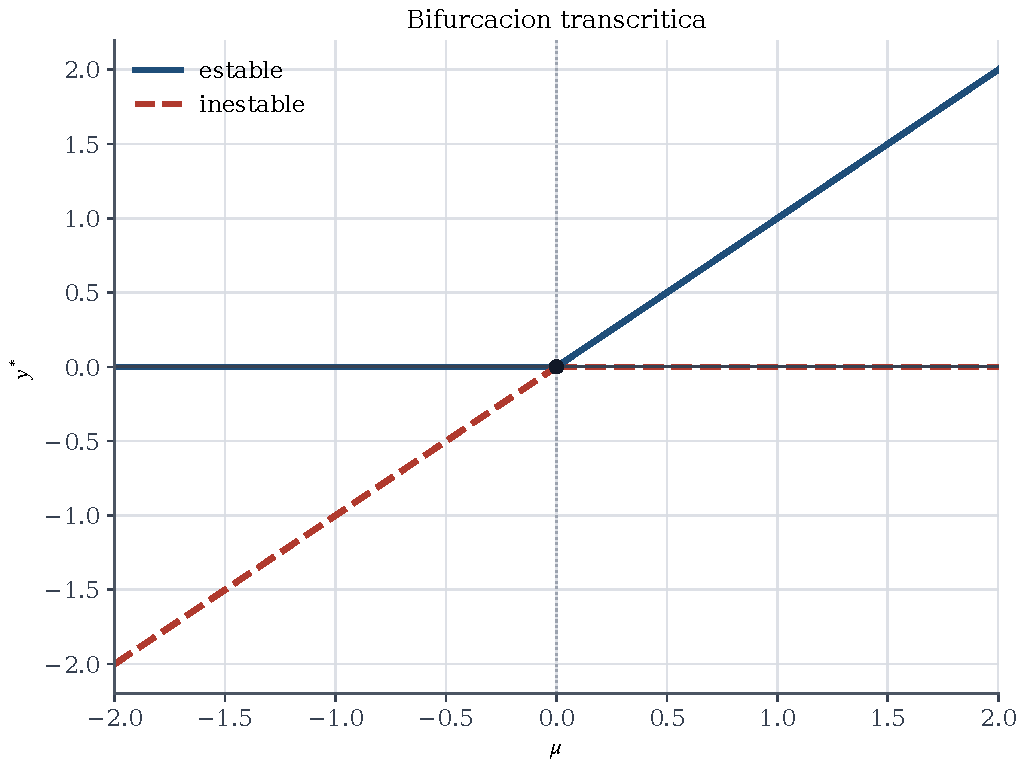
\includegraphics[width=0.80\textwidth]{figs/bif_c_transcritic.pdf}
  \caption{Diagrama de bifurcación para $\dot y=\mu y-y^2$. Las ramas $y^*=0$ y $y^*=\mu$ se intersectan en el origen e intercambian estabilidad al cruzar $\mu=0$.}
\end{figure}

\bigskip
\noindent\textbf{d)} $\displaystyle\frac{dy}{dx}=y(\mu-y^2)$ \quad (pitchfork supercrítica).

\textbf{Equilibrios.} $y^*=0$ y (para $\mu>0$) $y^*=\pm\sqrt{\mu}$.

\textbf{Linealización.} $f'(y)=\mu-3y^2$.
Idéntico al caso a): $f'(0)=\mu$; $f'(\pm\sqrt{\mu})=-2\mu<0$.
La bifurcación ocurre en $\mu=0$ con la misma estructura que a).

\textbf{Observación.} El factor $y$ hace que $y^*=0$ sea siempre equilibrio;
la factorización $y(\mu-y^2)$ muestra que la estructura es la misma
que $\mu y-y^3$ del caso a). El diagrama de bifurcación es idéntico.

\begin{figure}[H]
  \centering
  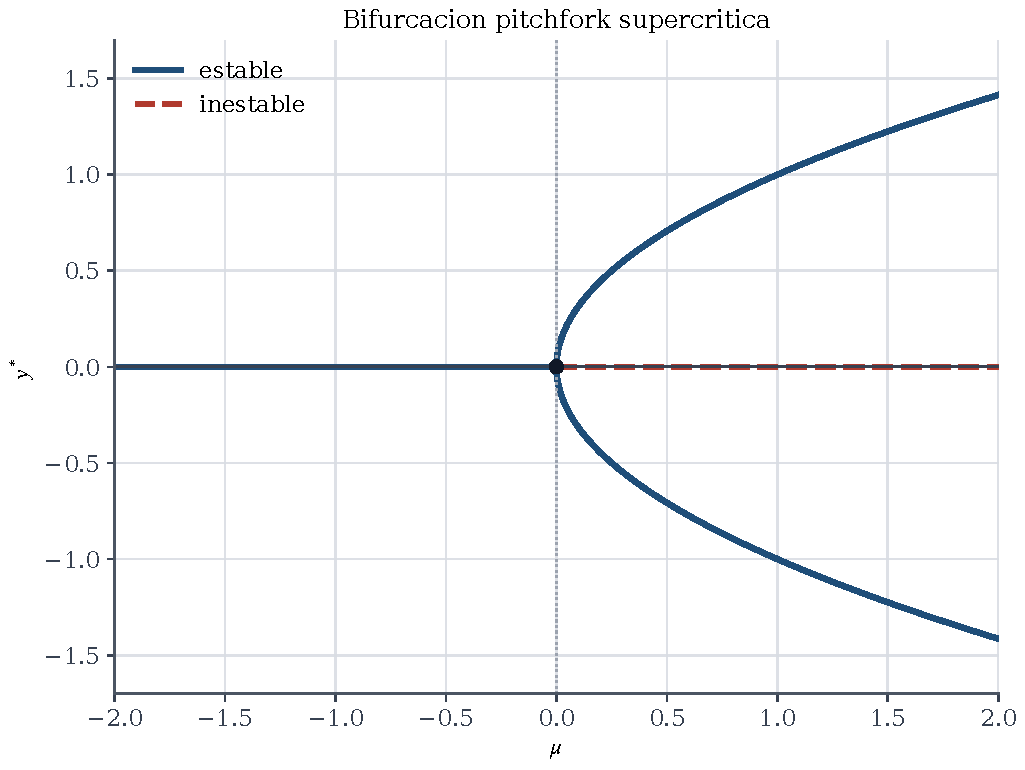
\includegraphics[width=0.80\textwidth]{figs/bif_d_pitchfork_sup2.pdf}
  \caption{Diagrama de bifurcación para $\dot y=y(\mu-y^2)$. La estructura es la misma que en el inciso a): la rama $y^*=0$ cambia de estable a inestable en $\mu=0$ y emergen dos ramas estables no triviales.}
\end{figure}

\bigskip
\noindent\textbf{f)} $\displaystyle\frac{dy}{dx}=y^2+\mu$ \quad (silla-nodo).

\textbf{Equilibrios.} $y^2+\mu=0\;\Rightarrow\; y^*=\pm\sqrt{-\mu}$ solo para $\mu<0$.

\textbf{Linealización.} $f'(y)=2y$.
\[
  f'(-\sqrt{-\mu})=-2\sqrt{-\mu}<0\;\Rightarrow\; y^*=-\sqrt{-\mu} \text{ estable}.
\]
\[
  f'(\sqrt{-\mu})=2\sqrt{-\mu}>0\;\Rightarrow\; y^*=\sqrt{-\mu} \text{ inestable}.
\]
En $\mu=0$: único equilibrio $y^*=0$ con $f'(0)=0$ (semiestable; linealización no decide).
Para $\mu>0$: no hay equilibrios reales.

\textbf{Bifurcación.} En $\mu=0$ los dos equilibrios colisionan y desaparecen
(bifurcación silla-nodo).

\begin{figure}[H]
  \centering
  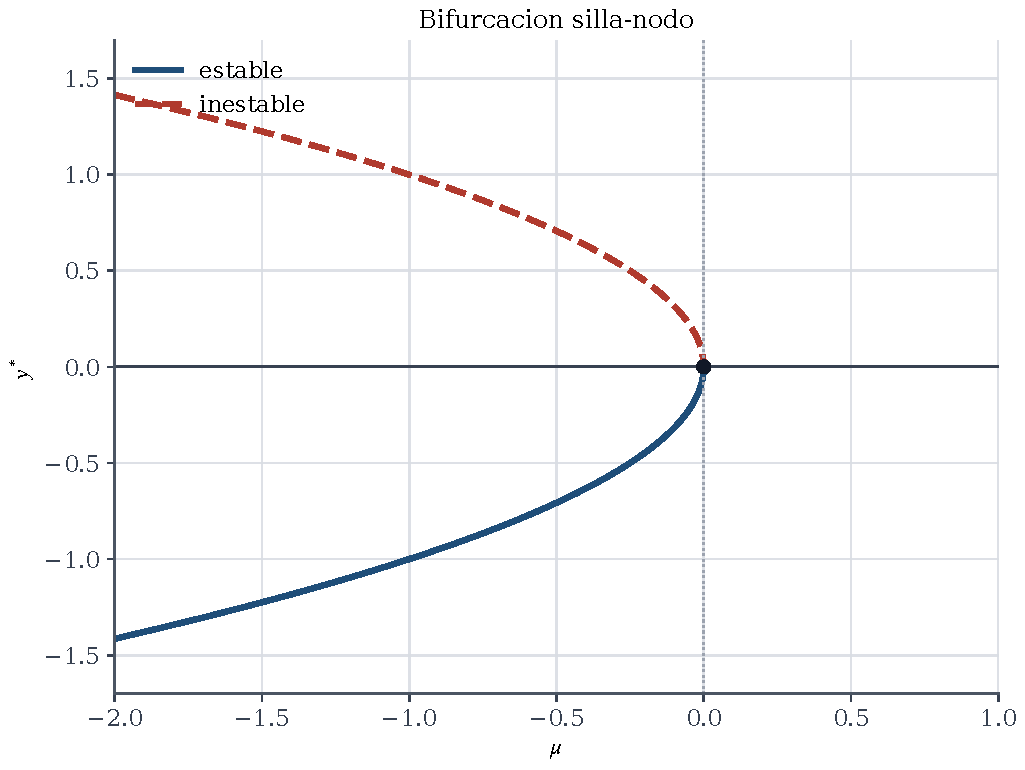
\includegraphics[width=0.80\textwidth]{figs/bif_f_saddle_node.pdf}
  \caption{Diagrama de bifurcación para $\dot y=y^2+\mu$. Cuando $\mu<0$ aparecen dos equilibrios, uno estable y uno inestable, que colisionan en $\mu=0$ y desaparecen para $\mu>0$.}
\end{figure}

\bigskip
\noindent\textbf{g)} $\displaystyle\frac{dy}{dx}=\mu y+y^3$ \quad (pitchfork subcrítica).

\textbf{Equilibrios.} $y(\mu+y^2)=0\;\Rightarrow\; y^*=0$ y (para $\mu<0$) $y^*=\pm\sqrt{-\mu}$.

\textbf{Linealización.} $f'(y)=\mu+3y^2$.
\[
  f'(0)=\mu:\quad
  \begin{cases}
    \mu<0: & y^*=0 \text{ estable},\\
    \mu>0: & y^*=0 \text{ inestable}.
  \end{cases}
\]
Para $\mu<0$: $f'(\pm\sqrt{-\mu})=\mu+3(-\mu)=-2\mu>0$,
luego $y^*=\pm\sqrt{-\mu}$ son \emph{inestables}.

\textbf{Diagrama de bifurcación.}
Para $\mu<0$: $y^*=0$ estable y $y^*=\pm\sqrt{-\mu}$ inestables.
En $\mu=0$: bifurcación subcrítica; $y^*=\pm\sqrt{-\mu}\to 0$.
Para $\mu>0$: solo $y^*=0$, pero es inestable.
La presencia de ramas inestables para $\mu<0$ produce \emph{histéresis}.

\begin{figure}[H]
  \centering
  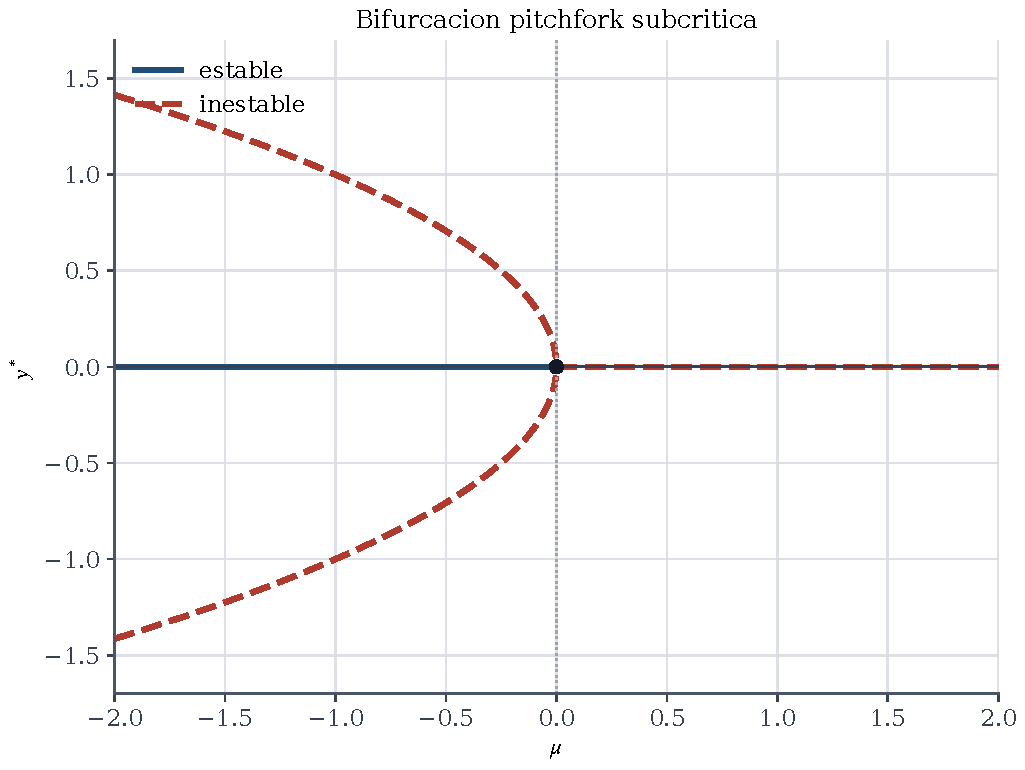
\includegraphics[width=0.80\textwidth]{figs/bif_g_pitchfork_sub.pdf}
  \caption{Diagrama de bifurcación para $\dot y=\mu y+y^3$. La rama trivial es estable para $\mu<0$ e inestable para $\mu>0$, mientras que las ramas no triviales existen solo para $\mu<0$ y son inestables.}
\end{figure}

\bigskip
\noindent\textbf{h)} $\displaystyle\frac{dy}{dx}=y(\mu-y)$ \quad (transcrítica).

\textbf{Equilibrios.} $y^*=0$ y $y^*=\mu$ para todo $\mu$.

\textbf{Linealización.} $f'(y)=\mu-2y$.
\[
  f'(0)=\mu,\qquad f'(\mu)=-\mu.
\]
Para $\mu<0$: $y^*=0$ estable, $y^*=\mu$ inestable.
Para $\mu>0$: $y^*=0$ inestable, $y^*=\mu$ estable.
En $\mu=0$: ambos equilibrios coinciden; intercambio de estabilidad.

\textbf{Nota.} El caso h) es algebraicamente idéntico al caso c)
($y'=\mu y-y^2=y(\mu-y)$). Los diagramas de bifurcación son el mismo.

\begin{figure}[H]
  \centering
  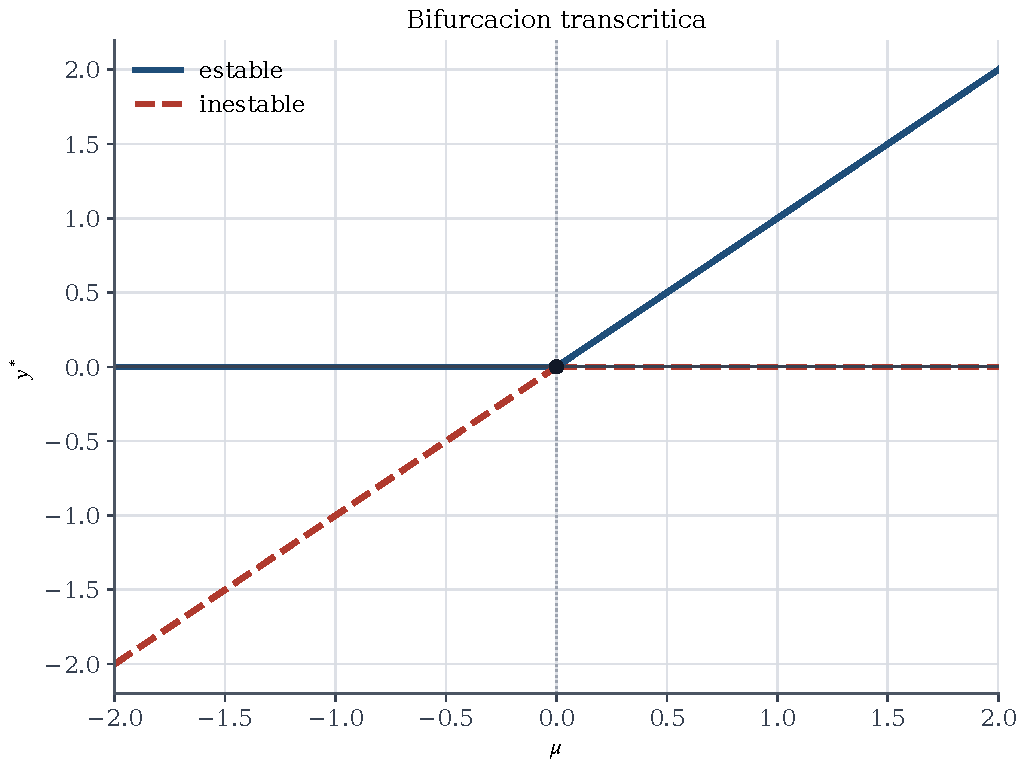
\includegraphics[width=0.80\textwidth]{figs/bif_h_transcritic2.pdf}
  \caption{Diagrama de bifurcación para $\dot y=y(\mu-y)$. Como en el inciso c), las ramas se cruzan en el origen y la estabilidad se intercambia al cambiar el signo de $\mu$.}
\end{figure}

\bigskip
\noindent\textbf{i)} $\displaystyle\frac{dy}{dx}=\mu\sin(y)$ \quad (bifurcación periódica).

\textbf{Equilibrios.} $\mu\sin(y^*)=0\;\Rightarrow\; y^*=k\pi$, $k\in\mathbb{Z}$,
para todo $\mu\neq 0$.
Para $\mu=0$: todo punto es equilibrio.

\textbf{Linealización.} $f'(y)=\mu\cos(y)$.
\[
  f'(k\pi)=\mu\cos(k\pi)=\mu(-1)^k.
\]
Para $\mu>0$:
$k$ par ($y^*=0,\pm 2\pi,\ldots$): $f'=\mu>0$, \emph{inestables}.
$k$ impar ($y^*=\pm\pi,\pm 3\pi,\ldots$): $f'=-\mu<0$, \emph{estables}.

Para $\mu<0$: estabilidades invertidas.

En $\mu=0$: bifurcación donde todos los equilibrios tienen $f'=0$.
Al cruzar $\mu=0$ todos los equilibrios intercambian estabilidad simultáneamente.

\textbf{Diagrama de bifurcación.}
Para cada entero $k$, la rama $y^*=k\pi$ es horizontal en el diagrama $(\mu,y^*)$.
Las ramas con $k$ par son estables para $\mu<0$ e inestables para $\mu>0$;
las de $k$ impar, al revés. La estructura se repite periódicamente en $y$.

\begin{figure}[H]
  \centering
  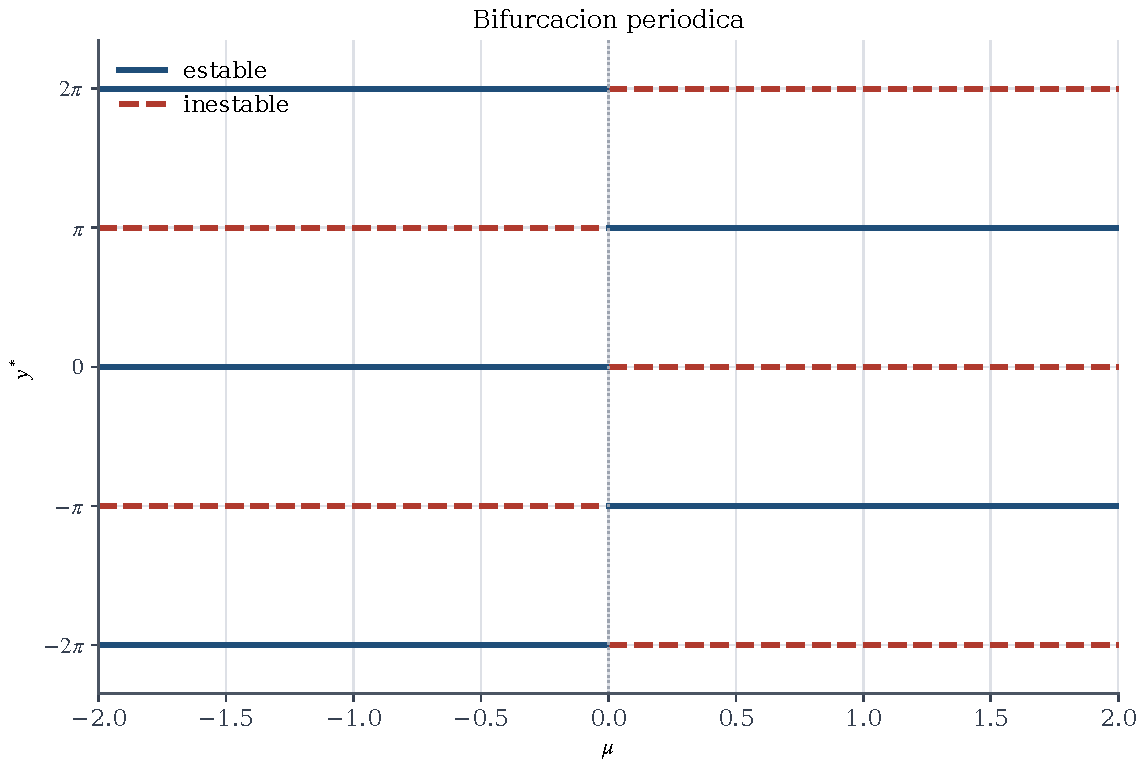
\includegraphics[width=0.88\textwidth]{figs/bif_i_periodica.pdf}
  \caption{Diagrama de bifurcación para $\dot y=\mu\sin(y)$, mostrando varias ramas periódicas de equilibrios. Al cruzar $\mu=0$ todas las ramas intercambian estabilidad de manera simultánea.}
\end{figure}

\bigskip
\noindent\textbf{j)} $\displaystyle\frac{dy}{dx}=y^3-3\mu y+\mu$ \quad (cúspide, codimensión 2).

\textbf{Reescritura.} Definiendo
\[
  r=3\mu,\qquad h=\mu,
\]
la familia puede escribirse como
\[
  \dot y = y^3-r y+h.
\]
Esto corresponde a una sección uniparamétrica de la forma normal de la
bifurcación cúspide: al variar $\mu$, se recorre la recta $(r,h)=(3\mu,\mu)$
en el plano de parámetros.

\textbf{Equilibrios.} Los puntos fijos satisfacen:
\[
  y^3-3\mu y+\mu=0.
\]
Esta ecuación cúbica puede tener 1 o 3 raíces reales según el valor de $\mu$.
El discriminante de $p(y)=y^3-3\mu y+\mu$ es $\Delta=4(3\mu)^3-27\mu^2=108\mu^3-27\mu^2=27\mu^2(4\mu-1)$.

\begin{itemize}
  \item $\mu<0$: $\Delta<0$, una sola raíz real.
  \item $\mu=0$: $p(y)=0$ implica $y=0$ (raíz triple degenerada); $\Delta=0$.
  \item $0<\mu<1/4$: $\Delta<0$, una sola raíz real.
  \item $\mu=1/4$: $\Delta=0$, bifurcación silla-nodo; dos equilibrios coinciden.
  \item $\mu>1/4$: $\Delta>0$, tres raíces reales.
\end{itemize}

\textbf{Linealización.} $f'(y)=3y^2-3\mu=3(y^2-\mu)$.
Como en un sistema unidimensional un equilibrio es estable cuando $f'(y^*)<0$,
se concluye que $y^*$ es estable si $y^{*2}<\mu$ e inestable si $y^{*2}>\mu$.
Por tanto, cuando existen tres equilibrios, la rama central es estable y las
dos ramas exteriores son inestables.

\textbf{Bifurcación.} El valor $\mu=0$ produce un equilibrio triple en $y=0$,
que corresponde al punto degenerado donde la trayectoria paramétrica pasa por
el vértice de la cúspide. Además, en $\mu=1/4$ ocurre una bifurcación
silla-nodo, pues el polinomio es tangente al eje horizontal y aparecen dos
ramas adicionales de equilibrio.

\textbf{Naturaleza codimensión 2.} La cúspide requiere dos parámetros libres
para describir toda su geometría en el plano $(r,h)$. En este ejercicio,
sin embargo, se estudia solo la recta $(r,h)=(3\mu,\mu)$; por eso se observa
una familia uniparamétrica que entra en la región de tres equilibrios cuando
$\mu>1/4$.

\begin{figure}[H]
  \centering
  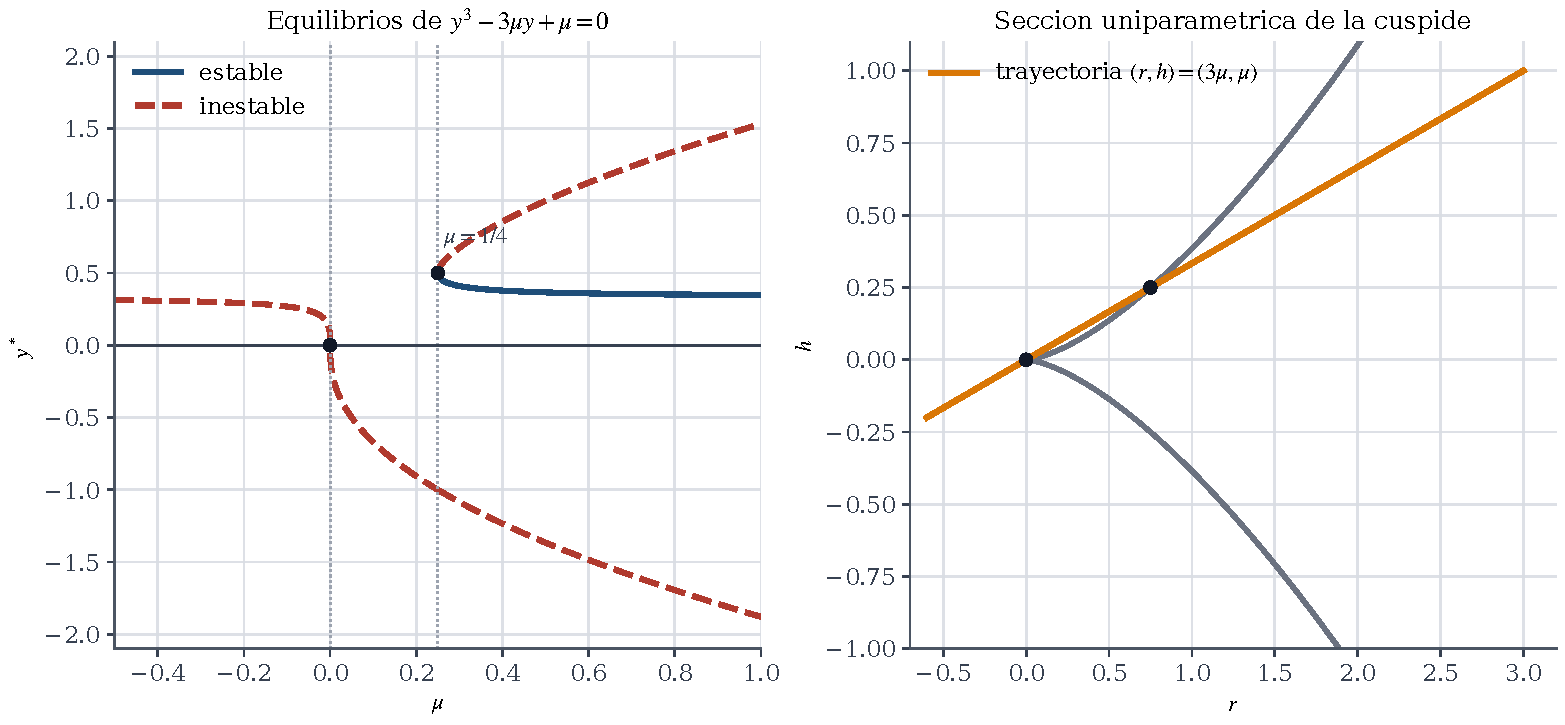
\includegraphics[width=0.96\textwidth]{figs/bif_j_cusp.pdf}
  \caption{A la izquierda se muestra el diagrama de equilibrios de $\dot y=y^3-3\mu y+\mu$ en función de $\mu$, donde para $\mu>1/4$ aparecen tres ramas y la rama central es estable. A la derecha se representa la trayectoria paramétrica $(r,h)=(3\mu,\mu)$ dentro del diagrama de cúspide asociado.}
\end{figure}

\bigskip
\noindent\rule{\textwidth}{0.3pt}

\end{document}
